\chapter{Belle to Belle II Format Conversion}

\section{Conversion Procedure}
The Belle experiment finished its data-taking run of 10 years at the end of 2010 after collecting a dataset of about $1\e{ab^{-1}}$. That year the Belle detector was shut down and the Belle II experiment has started in its place. While the focus moved to the construction of the Belle II detector and the development of the Belle II Analysis Framework (BASF2) \cite{Kuhr:2018lps}, Belle analyses are still on-going and Belle data is still being used today. BASF2 software with its modular structure has a more intuitive approach to performing analyses, however, since it was rewritten completely from scratch, it was designed for the incoming Belle II data and therefore out-of-the-box usage of Belle data is outside of its scope.

In the Belle II Collaboration, a task force was created in order to convert Belle data into Belle II format (\btbii) \cite{Keck:b2bii2018}. The \btbii~package was developed as a part of BASF2 in order to convert data and MC of the Belle experiment and make it available within BASF2. In addition to the convenience of Belle data being processed in the more intuitive and advanced BASF2 framework, \btbii~allows for estimation and validation of performances of various advanced algorithms being developed for Belle II. The conversion itself, however, is considered non-trivial. Although the conversion of the raw detector data would be possible, the reconstruction algorithms of BASF2 are optimized for Belle II and cannot be effectively applied to Belle data. To bypass this problem, reconstructed objects from \texttt{PANTHER} tables, a custom solution of the Belle collaboration based on C/C++ and Fortran, are mapped to their corresponding representations in BASF2. In this analysis, we use the developed converter package in order to analyze Belle data with the Belle II software.

The conversion in the \btbii~package is divided into three BASF2 modules. The first module opens the Belle input files and reads the events into memory in the form of \texttt{PANTHER} tables. This module consists predominantly of reused BASF code. The second module applies various calibration factors, such as experiment- and run-dependent factors, to the beam energy, particle identification information, error matrices of the fitted tracks, etc. The module also applies some low-level cuts to reproduce removing background events as done within BASF. The actual conversion and the mapping of reconstructed objects are done in the last module. For more information see \cite{Keck:48940}.

\section{Validation}

In order to make sure the conversion was successful and without errors, a thorough validation should be performed. This is done by comparing histograms of all physical quantities of the reconstructed objects on simulated and recorded events, processed with BASF and BASF2. 

Our signal decay mode consists of three charged tracks, track conversion should perform flawlessly. Additionally, energy measurement is also very important in our untagged analysis in order to successfully determine the missing 4-momentum in the event, which is why we also need a correct conversion of the ECL clusters for photons and $\pi^0$ particles. Figures \ref{fig:b2bii_tracks} to \ref{fig:b2bii_pi0s} show the basic physical properties of converted tracks, photons and $\pi^0$ particles, obtained with BASF and BASF2, and their difference, which is (up to numerical precision) equal to 0. The plots indicate that the conversion is successful in all aspects and we can proceed with the analysis in the framework of BASF2.

\begin{figure}[H]
	\centering
	\captionsetup{width=0.8\linewidth}
	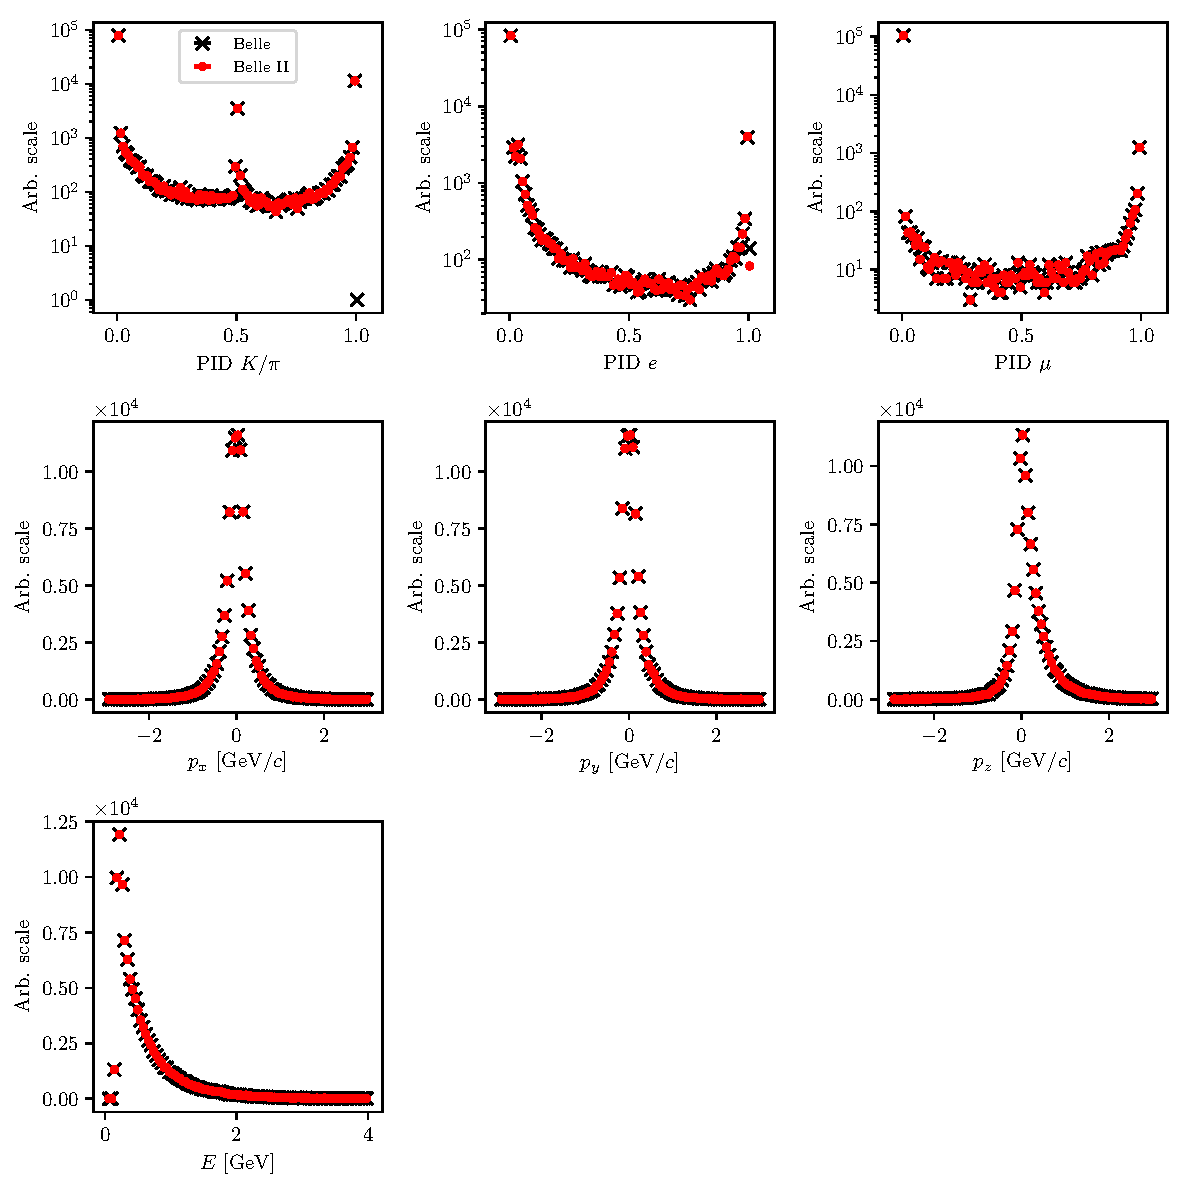
\includegraphics[width=\linewidth]{fig/b2bii_tracks}
	\caption{Some of the more important physical properties of tracks for Belle and Belle II in the conversion process. The histograms seem to overlap and the conversion is assumed to be successful.}
	\label{fig:b2bii_tracks}
\end{figure}

\begin{figure}[H]
	\centering
	\captionsetup{width=0.8\linewidth}
	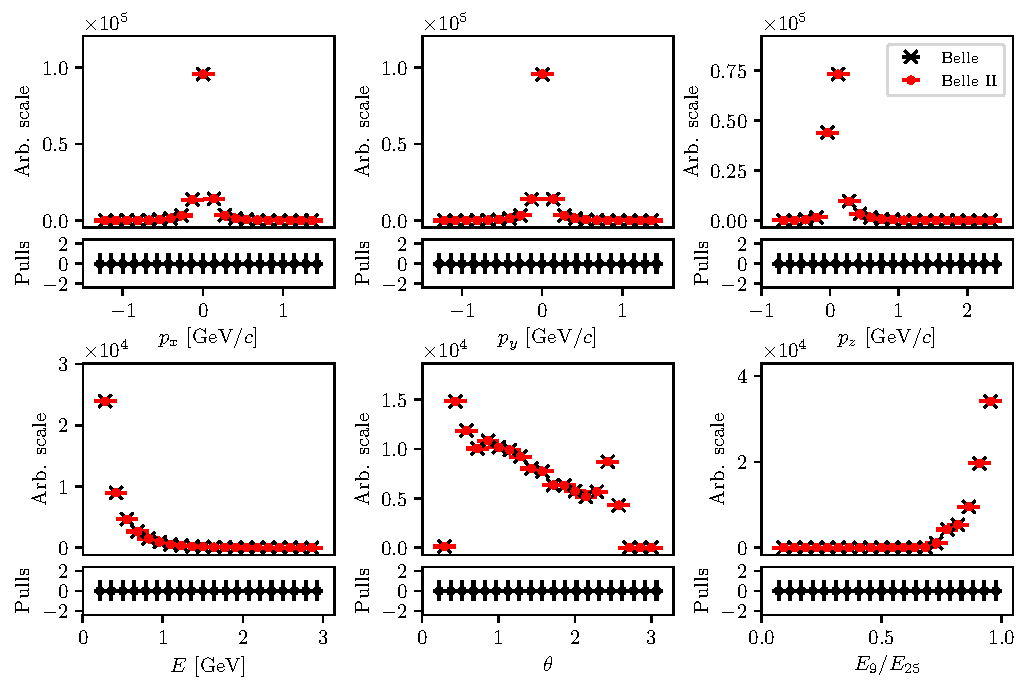
\includegraphics[width=\linewidth]{fig/b2bii_gammas}
	\caption{Some of the more important physical properties of photons for Belle and Belle II in the conversion process. The histograms seem to overlap and the conversion is assumed to be successful.}
	\label{fig:b2bii_gammas}
\end{figure}

\begin{figure}[H]
	\centering
	\captionsetup{width=0.8\linewidth}
	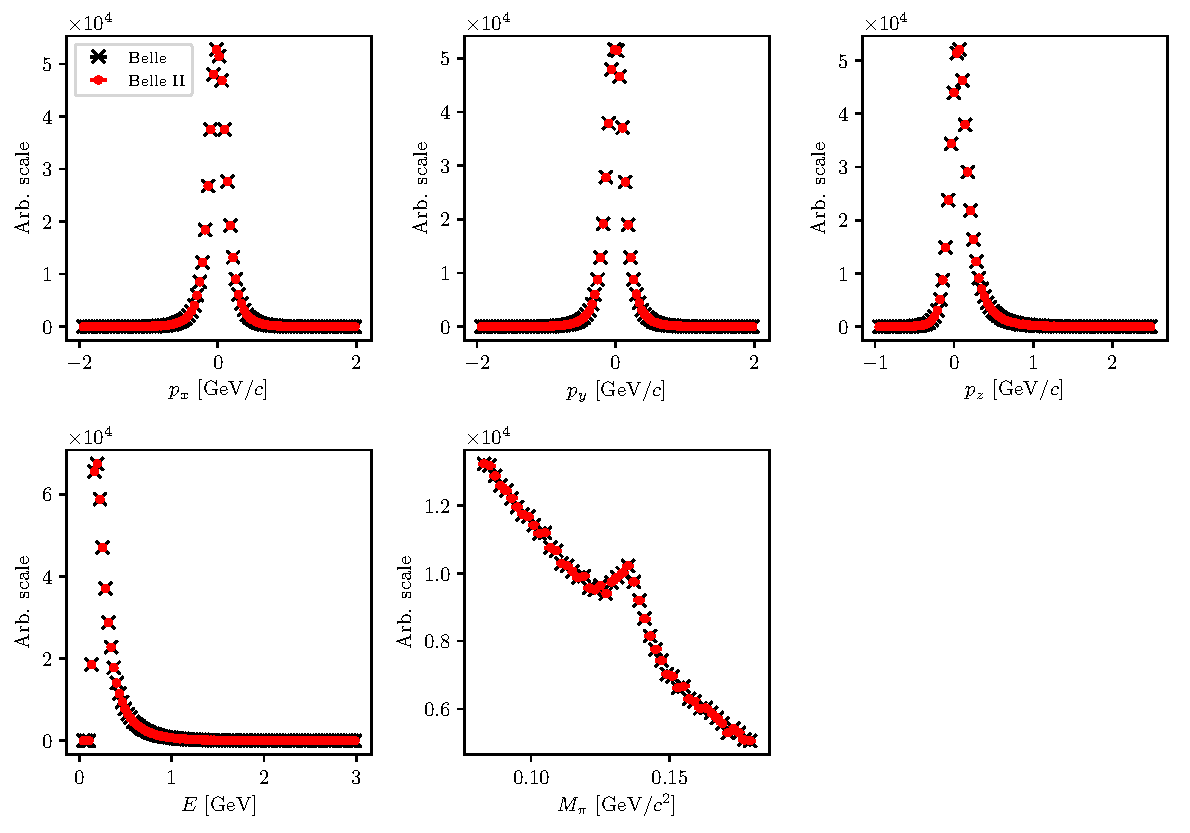
\includegraphics[width=\linewidth]{fig/b2bii_pi0s}
	\caption{Some of the more important physical properties of $\pi^0$ particles for Belle and Belle II in the conversion process. The histograms seem to overlap and the conversion is assumed to be successful.}
	\label{fig:b2bii_pi0s}
\end{figure}

%\section{Conversion improvement}
%
%An additional improvement is applied to neutral particles after the conversion where we change the origin of the ECL clusters to the interaction point instead of the point $(0,0,0)$, which was used at Belle. In order to successfully implement this improvement, we have to make sure that the conversion of the beam parameters is successful and how the momentum resolution of neutral particles changes after its implementation. Figure X shows the distributions of the beam parameters for Belle and Belle II, which shows no obvious errors in the conversion process. Improving the information about the origin point of photons then results in improvement of the momentum determination. The comparison is shown in Figure X with an obvious benefit after the mentioned implementation.
%
%PLOT
%
%PLOT